% TO RUN THE GIF, YOU NEED ADOBE READER!

\sisetup{locale = EN} 
\title{\textbf{\rmfamily Introduction to Data Analysis}}
\subtitle{Histograms, Filters, Invariant Mass}
\author[~\PersonDataAnalysis~]{{\PersonDataAnalysis}}
\institute[\WorkGroup]{ \University}
\date{\dateMC}
%%%%%%%%%%%%%%%%%%%%%%%%%%%%%%%%%%%%%%%%%%%%%%%%%%%%%%%%%%%%%%%%%%%%%%%%%%%%%%%%%%%%%%%%%%%%%%
%   Options for the footline
%%%%%%%%%%%%%%%%%%%%%%%%%%%%%%%%%%%%%%%%%%%%%%%%%%%%%%%%%%%%%%%%%%%%%%%%%%%%%%%%%%%%%%%%%%%%%%
\setbeamertemplate{footline}
{
\leavevmode%
\hbox{%
\begin{beamercolorbox}[wd=0.5\paperwidth,ht=2.25ex,dp=1ex,center]{author in foot}%
\usebeamerfont{author in foot} \parbox{0.5\paperwidth}{\insertsubsection{}}
\end{beamercolorbox}%
\begin{beamercolorbox}[wd=0.11\paperwidth,ht=2.25ex,dp=1ex,center]{title in head/foot}%
\usebeamerfont{title in head/foot}
\end{beamercolorbox}%
\begin{beamercolorbox}[wd=0.385\paperwidth,ht=2.25ex,dp=1ex,right]{date in head/foot}%
\usebeamerfont{date in head/foot}\insertsection{}\hfill
|~Slide \insertframenumber{} \hspace*{2ex}%/ \inserttotalframenumber\hspace*{2ex}
\end{beamercolorbox}}%
\vskip0pt%
}
\tikzset{>=latex}
\usetikzlibrary{decorations.markings, calc}
\newcommand{\midlabelline}[3]{
   \node (midlabel) at ($ (#1)!.5!(#2) $) {#3};
   \draw[<-] (#1) --  (midlabel);
   \draw[->] (midlabel) -- (#2);}


\begin{document}\selectlanguage{english}
%%%%%%%%%%%%%%%%%%%%%%%%%%%%%%%%%%%%%%%%%%%%%%%%%%%%%%%%%%%%%%%%%%%%%%%%%%%%%%%%%%%%%%%%%%%%%%
\begin{frame}[plain]
\begin{center}
    \begin{tabular}{ccc}
 \parbox{0.33\textwidth}{\LogoInsitute}    &
 ~~~~\parbox{0.33\textwidth}{\includegraphics[height=1cm]{Logos And Group/LHCb_Logo.png}}   &  \parbox{0.33\textwidth}{\LogoUniversity}\\
\end{tabular}
\end{center}

\maketitle
\end{frame}
\section{Introduction}
\begin{frame}
  We want to find a new particle!\\ 
\begin{minipage}{0.25\textwidth}
~
\end{minipage}
\begin{minipage}{0.48\textwidth}
 \begin{center}
 \Large    \[\mathbf{\Omega_c^0 \rightarrow \Xi_c^+ \, K^-}\]
    \includegraphics[0.7\textwidth]{Figures Lecture on Datanalysis/penguin2.jpeg}
\end{center} 
\end{minipage}
\begin{minipage}{0.25\textwidth}
    Quark content:\\
    \begin{tabular}{cc}
        $\Omega_c^0$ & $ssc$  \\
         $\Xi^+$ & $usc$ \\ 
         $K^-$ & $s \bar u$
    \end{tabular}
\end{minipage}
      
   \normalsize \ding{43} How can we search for the $\Omega_c^0$?
\end{frame}
%%%%%%%%%%%%%%%%%%%%%%%%%%%%%%%%%%%%%%%%%%%%%%%%%%%%%%%%%%%%%%%%%%%%%%%%%%%%%%%%%%%%%%%%%%%%%%
\section{Mass concept}

%%%%%%%%%%%%%%%%%%%%%%%%%%%%%%%%%%%%%%%%%%%%%%%%%%%%%%%%%%%%%%%%%%%%%%%%%%%%%%%%%%%%%%%%%%%%%%
   \begin{frame}
   \begin{center} \begin{spacing}{2}
       \Large The term \\ \LARGE \textbf{Mass} \\ \Large in our everyday's language
   \end{spacing}\end{center}
   
   \end{frame}
   %%%%%%%%%%%%%%%%%%%%%%%%%%%%%%%%%%%%%%%%%%%%%%%%%%%%%%%%%%%%%%%%%%%%%%%%%%%%%%%%%%%%%%%%%%%%%%
   \subsection{Picture: Airbus}
\begin{frame}{Let me Ask you...}
\begin{minipage}{0.1\textwidth}
    \quad
\end{minipage}
            \begin{minipage}[t]{0.49\textwidth}
      \vspace{1cm} 
      What properties do you associate with \emph{mass}? %\pause \\ Our ideas:
      
      \begin{center}
        \begin{itemize}
             \item[-] long-lasting
            \item [-] extended
            \item [-]‘there’
            \item [-] Easily detectable
        \end{itemize}
         \end{center}
      \end{minipage}
      \begin{minipage}[t]{0.29\textwidth}
     \centering
     \vspace{+.1cm}
         \includegraphics[width=2cm]{Figures Lecture on Hadrons/SevenMountainsMilk.png}\\ \vspace{.5cm}
         \includegraphics[width=2.5cm]{Figures Lecture on Hadrons/Airbus A321Neo.jpg}
           \end{minipage} 
 \end{frame}
 %%%%%%%%%%%%%%%%%%%%%%%%%%%%%%%%%%%%%%%%%%%%%%%%%%%%%%%%%%%%%%%%%%%%%%%%%%%%%%%%%%%%%%%%%%%%%%
\begin{frame}{What are we Dealing with?}
\begin{minipage}[t]{0.39\textwidth}
     \centering
     \vspace{+.4cm}
        \begin{tikzpicture}[yscale = 1.2,xscale=0.6]\tiny



\draw[fill=LHCbLightBlue!80] (4.7,2) to (3.6,2.2)  to (2.5,2.4)  to (1.4,2.6)to (3.6,2.7) to(5.8,2.8)  to  (8.0,2.9)to(6.9,2.6)    to(5.8,2.3)   to(4.7,2);
\draw[fill=LHCbLightBlue!80] (4.8,3) node [below left=-2pt] {\textcolor{black}{$\mathbf{\Omega_{c}^{0}}$}} to (3.7,3.20) to (2.6,3.4) to(4.58,3.49) to (7,3.6)  to(5.9,3.3) node [below right] {\textcolor{black}{$\mathbf{\Xi_{c}^{+}}$}}  to(4.8,3);
    \draw[fill=LHCbLightBlue!80] (6,4.3)  to (4.9,4) to (3.8,4.2) to (6,4.3);
\draw[black, --] (5,5) to (4.9,4)  to (4.8,3)   node [above=2pt] {\colorbox{LHCbLightBlue!80}{$ssc$}}  to (4.7,2)   (5,5)to(6,4.3)   to(7,3.6)  to(8.0,2.9)   (5,5)to(3.8,4.2) to(2.6,3.4)  to(1.4,2.6)   ;
\draw[](5.9,3.3) node [above left=-1pt] {\tiny $usc$};
 \node (ccc) at (5,5) {$\bullet$};
        
        \node (scc) at (4.9,4) {$\bullet$};
        \node (ucc) at (6,4.3) {$\bullet$};
        \node (dcc) at (3.8,4.2) {$\bullet$};
        
         \node (ssc) at (4.8,3) {$\bullet$};
         \node (dsc) at (3.7,3.20) {$\bullet$};
         \node (ddc) at (2.6,3.4) {$\bullet$};
             \node (usc) at (5.9,3.3) {$\bullet$};
             \node (uuc) at (7,3.6) {$\bullet$};

         
          \node (sss) at (4.7,2) {$\bullet$};
          \node (dss) at (3.6,2.2) {$\bullet$};
          \node (uds) at (4.63,2.53) {$\bullet$} ;
          \node (dds) at (2.5,2.4) {$\bullet$};
          \node (ddd) at (1.4,2.6) {$\bullet$};
                    \node (uss) at (5.8,2.3) {$\bullet$};
                     \node (uus) at (6.9,2.6) {$\bullet$};
                     \node (uuu) at (8.0,2.9) {$\bullet$};

      \node (udc) at (4.58,3.49) {$\bullet$};
      \node (udd) at (3.6,2.7) {$\bullet$};
      \node (uud) at (5.8,2.8) {$\bullet$};

    \end{tikzpicture}
Heavy baryons
           \end{minipage}
            \begin{minipage}[t]{0.59\textwidth}
Which of these applies to heavy hadrons? %%\pause %Schwer niemals definiert 
\begin{center}
        \begin{itemize}
            \item[-] Unstable, decaying
            \item[-] Short-lived
            \item[-] Small {\small(atomic nuclei $\sim 10^{-14}\,$m})
            \item[-] Must be generated
            \item [$\Rightarrow$] \textbf{Not easily detectable}
            \\\item [\,] %\pause
            \item [\ding{43}] Ideas?
        \end{itemize}
        \end{center}
      \end{minipage}
    \end{frame}
    \subsection{}
%%%%%%%%%%%%%%%%%%%%%%%%%%%%%%%%%%%%%%%%%%%%%%%%%%%%%%%%%%%%%%%%%%%%%%%%%%%%%%%%%%%%%%%%%%%%%%

\begin{frame}{Search for $\Omega_c^0$}

  \begin{center} \vspace{-1cm}
 \Large    \[\mathbf{\Omega_c^0 \rightarrow \Xi_c^+ \, K^-}\]
 \end{center}
   \begin{spacing}{1.5}
       
  
    \begin{itemize}    \item[\ding{202}] \textbf{ Search for the decay products in the LHCb data }
    \item[] \textcolor{white}{Combine the decay products and look at the mass spectrum }
    \item[] \textcolor{white}{If we find a peak, we have discovered a new particle! }
\end{itemize}
 \end{spacing}

\end{frame}
\begin{frame}{$\Omega_c^0$ Decay}
Quark content of $\Omega_c^0:~~css$
\vspace{0.5cm}
\begin{center}
\begin{tikzpicture}
\begin{feynman}
    \vertex(cl) {\(c\)};
    \vertex[right=5cm of cl] (cr) {\(c\)};
    \vertex[below=1cm of cl] (sl1) {\(s\)};
    \vertex[right=5cm of sl1] (sr1) {\(s\)};
    \vertex[below right = 1cm and 2cm of cl] (g1);
    \vertex[below right = 1cm and 1.5cm of g1] (g2);
    \vertex[below = 0.5cm of sr1] (u) {\(u\)};
    \vertex[below = 1cm of u] (ubar) {\(\bar u\)};
    \vertex[below=2cm of sl1] (sl2) {\(s\)};
    \vertex[right=5cm of sl2] (sr2) {\(s\)};
    \diagram* { {[edges=fermion]
    (cl) -- (cr), (sl1) -- (g1), (g1) -- (sr1),
    (sl2) -- (sr2), (g2) -- (u), (ubar) -- (g2)};
    (g1) -- [boson, edge label = \(g\)] (g2)
    };
\draw [decoration={brace}, decorate] (sl2.south west) -- (cl.north west) node [pos=0.5, left] {\(\Omega_c^0\)};
\draw [decoration={brace}, decorate] (cr.north east) --  (u.south east) node [pos=0.5, right] {\(\Xi_c^+\)};
\draw [decoration={brace}, decorate] (ubar.north east) --  (sr2.south east) node [pos=0.5, right] {\(K^-\)};
\end{feynman}
\end{tikzpicture}   
\end{center}
%%\pause

\\ %\pause
However, the $\Xi_c^+$ is not stable and decomposes further into \begin{center}
   \Large $\mathbf{\Xi_c^+ \rightarrow p\, K^-\, \boldsymbol \pi^+}$
\end{center}
\end{frame}
\begin{frame}
\frametitle{The $\Xi_c^+$ Decay}

We know the $\Xi_c^+$ with lifetime \[\tau_{\Xi_c^+}\approx 4.5 \times 10^{-13}\,\text{s}\]
\begin{center}
    \begin{overpic}[width=10cm]{Figures Lecture on Datanalysis/LHCb_Calculation_tracks only.png}
\put(100,42){$\pi^+$}
\put(100,33){$p$}
\put(100,27){$K^-$}
\put(100,1){$K^-$}
\put(3,20){$\rotatebox[]{135}{\rightarrow}\Omega_c^0 $}
\put(3,30){$\leftarrow~\Xi_c^+\rightarrow$}
\end{overpic}
\end{center}


\small From precise vertex reconstruction, we can use the \textbf{flight distance} of the $\Xi_c^+$ ($\sim$ mm to cm) as a filter!
\end{frame}
%%%%%%%%%%%%%%%%%%%%%%%%%%%%%%%%%%%%%%%%%%%%%%%%%%%%%%%%%%%%%%%%%%%%%%%%%%%%%%%%%%%%%%%%%%%%%%
\begin{frame}{The $\Xi_c^+$ Decay} 
Here we consider the decay \begin{center}
    $\Xi_c^+ \rightarrow p K^- \pi^+$
\end{center} %\pause
\textbf{\textcolor{red}{Why this one in particular?}}\\
Other options would be e.g.\\ 
\begin{minipage}{0.5\textwidth}
\begin{itemize}
    \item $\Xi_c^+ \rightarrow \Xi^0 \pi^+$
    \item $\Xi_c^+ \rightarrow p K^0$ 
\end{itemize}  
\vspace{1.5cm}
\end{minipage}
\begin{minipage}{0.49\textwidth}
\begin{tikzpicture}
\draw[](-3,-3)circle(0.141cm);
    \draw[--] (-3.1,-3.1)--(-2.9,-2.9);
    \draw[--] (-3.1,-2.9)--(-2.9,-3.1);


\draw[](-2,-3)circle(0.141cm);
    \draw[--] (-2.1,-3.1)--(-1.9,-2.9);
    \draw[--] (-2.1,-2.9)--(-1.9,-3.1);

\draw[](-1,-3)circle(0.141cm);
    \draw[--] (-1.1,-3.1)--(-0.9,-2.9);
    \draw[--] (-1.1,-2.9)--(-0.9,-3.1);

\draw[](-3,-2)circle(0.141cm);
    \draw[--] (-3.1,-2.1)--(-2.9,-1.9);
    \draw[--] (-3.1,-1.9)--(-2.9,-2.1);

\draw[] (-2,-2) node {$\Vec{B}$};
% \draw[](-2,-2)circle(0.141cm);
%     \draw[--] (-2.1,-2.1)--(-1.9,-1.9);
%     \draw[--] (-2.1,-1.9)--(-1.9,-2.1);

\draw[](-1,-2)circle(0.141cm);
    \draw[--] (-1.1,-2.1)--(-0.9,-1.9);
    \draw[--] (-1.1,-1.9)--(-0.9,-2.1);

\draw[](-3,-1)circle(0.141cm);
    \draw[--] (-3.1,-1.1)--(-2.9,-0.9);
    \draw[--] (-3.1,-0.9)--(-2.9,-1.1);

\draw[](-2,-1)circle(0.141cm);
    \draw[--] (-2.1,-1.1)--(-1.9,-0.9);
    \draw[--] (-2.1,-0.9)--(-1.9,-1.1);

 \draw[](-1,-1)circle(0.141cm);
    \draw[--] (-1.1,-1.1)--(-0.9,-0.9);
    \draw[--] (-1.1,-0.9)--(-0.9,-1.1);

\draw[](-3,-4)circle(0.141cm);
    \draw[--] (-3.1,-4.1)--(-2.9,-3.9);
    \draw[--] (-3.1,-3.9)--(-2.9,-4.1);

\draw[](-2,-4)circle(0.141cm);
    \draw[--] (-2.1,-4.1)--(-1.9,-3.9);
    \draw[--] (-2.1,-3.9)--(-1.9,-4.1);

 \draw[](-1,-4)circle(0.141cm);
    \draw[--] (-1.1,-4.1)--(-0.9,-3.9);
    \draw[--] (-1.1,-3.9)--(-0.9,-4.1);

 \draw[](-4,-4)circle(0.141cm);
    \draw[--] (-4.1,-4.1)--(-3.9,-3.9);
    \draw[--] (-4.1,-3.9)--(-3.9,-4.1);

    \draw[](-4,-3)circle(0.141cm);
    \draw[--] (-4.1,-3.1)--(-3.9,-2.9);
    \draw[--] (-4.1,-2.9)--(-3.9,-3.1);

\draw[](-4,-2)circle(0.141cm);
    \draw[--] (-4.1,-2.1)--(-3.9,-1.9);
    \draw[--] (-4.1,-1.9)--(-3.9,-2.1);

\draw[](-4,-1)circle(0.141cm);
    \draw[--] (-4.1,-1.1)--(-3.9,-0.9);
    \draw[--] (-4.1,-0.9)--(-3.9,-1.1);

\draw[->,red] (-2.75,-4.3)--(-2.74,-0.9) node[black,above] {$K^0$};
 \draw[blue] (-0.65,-2.3) --++ (90:0)  arc (90:180:2)   ;
 \draw[->, blue] (-0.65,-2.3)--(0,-2.3)node[black,right] {$K^-$};

\end{tikzpicture}
 
\end{minipage}

\end{frame}
%%%%%%%%%%%%%%%%%%%%%%%%%%%%%%%%%%%%%%%%%%%%%%%%%%%%%%%%%%%%%%%%%%%%%%%%%%%%%%%%%%%%%%%%%%%%%%
\begin{frame}{Invariant Mass}
    \textbf{strategy:}\\ Reconstruction via (sufficiently) stable decay products
    \begin{center}
    \begin{overpic}[width=10cm]{Figures Lecture on Datanalysis/LHCb_Calculation_tracks only.png}
\put(100,42){$\pi^+$}
\put(100,33){$p$}
\put(100,27){$K^-$}
\put(100,1){$K^-$}
\put(3,20){$\rotatebox[]{135}{\rightarrow} \textbf{?}$}
\put(3,30){$\leftarrow~\textbf{?} ~\rightarrow$}
\end{overpic}\end{center} %\pause
What el. charge will the particles behind the question marks have?
\end{frame}
%%%%%%%%%%%%%%%%%%%%%%%%%%%%%%%%%%%%%%%%%%%%%%%%%%%%%%%%%%%%%%%%%%%%%%%%%%%%%%%%%%%%%%%%%%%%%%
\newcommand\Bigbullet{\raisebox{-1.1mm}{\scalebox{2.5}{$\bullet$}}}
\definecolor{orange}{rgb}{0.96,0.48,0.16}
\definecolor{lightblue}{rgb}{0.33,0.61,0.86}
\definecolor{goodgreen}{rgb}{0.43,0.70,0.26}
\newcommand\BigbulletG{\raisebox{-2mm}{\scalebox{3.5}{$\bullet$}}}
\begin{frame}{Search for $\Omega_c^0$}

  \begin{center} \vspace{-1cm}
 \Large    \[\mathbf{\Omega_c^0 \rightarrow \Xi_c^+ \, K^-}\]
 \end{center}
   \begin{spacing}{1.5}
       
  
    \begin{itemize}    \item[\ding{202}] Search for the decay products in the LHCb data 
    \item[\ding{203}]\textbf {Combine the decay products and look at the mass spectrum }
        \item[] \textcolor{white}{We filter data}
    \item[] \textcolor{white}{If we find a peak, we have discovered a new particle! }
\end{itemize}
 \end{spacing}

\end{frame}

\begin{frame}{Invariant Mass}
\begin{center}
We consider the grey particle. It is at rest and has the \\ rest mass = rest energy $m_{inv}$

     \begin{overpic}[width=8cm]{Figures Lecture on Datanalysis/Invarint_Mass_1.png}\put (9,22.5){\parbox{1cm}{\textcolor{white}{$m_{inv}$\\ \footnotesize{$v=0$}}}} \end{overpic}
\end{center}


\textcolor{white}{The mass of \BigbulletG is completely divided into the momentum and mass of the products \Bigbullet\Bigbullet\Bigbullet. \\
    \\ $\Rightarrow$ Add energy and momentum vectors to obtain the mass of \emph{particle 1}!}
    \end{frame}
\begin{frame}{Invariant Mass}
\begin{center}
We look at the grey particle. It is at rest and has the \\ rest mass = rest energy $m_{inv}$

     \begin{overpic}[width=8cm]{Figures Lecture on Datanalysis/Invarint_Mass_2.png}
     
     \put (9,22.5){\parbox{1cm}{\textcolor{white}{$m_{inv}$\\ \footnotesize{$v=0$}}}} 
     \put (47.5,22.5){\parbox{1cm}{\textcolor{black}{$m_{inv}$\\ \footnotesize{$v=0$}}}} 
     \put (90,34){\parbox{1cm}{\textcolor{black}{$m_1$\\ \footnotesize{$v_1$}}}} 
     \put (92,20){\parbox{1cm}{\textcolor{black}{$m_2$\\ \footnotesize{$v_2$}}}} 
     \put (90,5){\parbox{1cm}{\textcolor{black}{$m_3$\\ \footnotesize{$v_3$}}}} 
          
\end{overpic}
\end{center}
The particle decomposes into three products. \\ \, \\ \, \\ \,
\end{frame}
\begin{frame}{Invariant Mass}
\begin{center}
We look at the grey particle. It is at rest and has the \\ rest mass = rest energy $m_{inv}$

     \begin{overpic}[width=8cm]{Figures Lecture on Datanalysis/Invarint_Mass_2.png}
     
     \put (9,22.5){\parbox{1cm}{\textcolor{white}{$m_{inv}$\\ \footnotesize{$v=0$}}}} 
     \put (47.5,22.5){\parbox{1cm}{\textcolor{black}{$m_{inv}$\\ \footnotesize{$v=0$}}}} 
     \put (90,34){\parbox{1cm}{\textcolor{black}{$m_1$\\ \footnotesize{$v_1$}}}} 
     \put (92,20){\parbox{1cm}{\textcolor{black}{$m_2$\\ \footnotesize{$v_2$}}}} 
     \put (90,5){\parbox{1cm}{\textcolor{black}{$m_3$\\ \footnotesize{$v_3$}}}} 
          
\end{overpic}
\end{center}
The mass of \textcolor{gray}{\BigbulletG} is completely divided into momentum and mass/\,energy of the products \textcolor{orange}{\Bigbullet}\textcolor{lightblue}{\Bigbullet}\textcolor{goodgreen}{\Bigbullet}. \\ %\pause
    \\ $\Rightarrow$ Add energy and momentum vectors to get the mass of \textcolor{gray}{\BigbulletG}!
\end{frame}
%%%%%%%%%%%%%%%%%%%%%%%%%%%%%%%%%%%%%%%%%%%%%%%%%%%%%%%%%%%%%%%%%%%%%%%%%%%%%%%%%%%%%%%%%%%%%%

%%%%%%%%%%%%%%%%%%%%%%%%%%%%%%%%%%%%%%%%%%%%%%%%%%%%%%%%%%%%%%%%%%%%%%%%%%%%%%%%%%%%%%%%%%%%%%
 \begin{frame}{Invariant Mass}
     A simple task?\\ \vspace{0.5cm} %\pause
     \begin{itemize}
         \item [\ding{43}] You have to hit exactly the products of the decay! \\ 
         \item [\ding{43}] Data must be filtered. 
               \end{itemize}\vspace{0.5cm} %\pause
           Indications for combinatorics: 
           
          \begin{itemise}
         \item [\ding{202}]conservation of charge
         \item [\ding{203}]Common intersection of the track
                    \end{itemise}
\end{frame}
\begin{frame}{Example: Hypothesis $\Xi_c^+ \rightarrow p K^- \pi^+$}
 The LHCb measures $p$, $K^-$, $\pi^+$, $\mu^-$, $\gamma$ \\ %\pause 
\begin{minipage}{.4\textwidth}
    

\begin{tabular}{cc}
   \includegraphics[width=.4\textwidth]{Figures Lecture on Datanalysis/OnOff_button.png}  & \parbox{.5\textwidth}{$\LARGE \pi^+ $  \\ \,}        \\
   \includegraphics[width=.4\textwidth]{Figures Lecture on Datanalysis/OnOff_button.png}  & \parbox{.5\textwidth}{$\LARGE K^- $  \\ \,}           \\
   \rotatebox[]{180}{\includegraphics[width=.4\textwidth]{Figures Lecture on Datanalysis/OnOff_button.png}}  & \parbox{.5\textwidth}{$\LARGE \gamma $  \\ \,}           \\
   \rotatebox[]{180}{\includegraphics[width=.4\textwidth]{Figures Lecture on Datanalysis/OnOff_button.png}}  & \parbox{.5\textwidth}{$\LARGE \mu^- $  \\ \,}           \\
\includegraphics[width=.4\textwidth]{Figures Lecture on Datanalysis/OnOff_button.png}  & \parbox{.5\textwidth}{$\LARGE p$  \\ \,}              \\
               
\end{tabular}
\end{minipage} 
\begin{minipage}{.58\textwidth}
    \begin{overpic}[width=6.3cm]{Figures Lecture on Datanalysis/Invarint_Mass_2.png}
     
     \put (11,22.5){\parbox{1cm}{\textcolor{white}{\footnotesize $\Xi_c^+$}}} 
     \put (49.75,22.5){\parbox{1cm}{\textcolor{black}{\footnotesize $\Xi_c^+$}}} 
     \put (81,35){\parbox{1cm}{\textcolor{black}{\footnotesize $\pi^+$}}} 
     \put (82,21){\parbox{1cm}{\textcolor{black}{\footnotesize $K^-$}}} 
     \put (83,6){\parbox{1cm}{\textcolor{black}{\footnotesize $p$}}} 
          
\end{overpic}\small  \\ 
Functionality of \textbf{\textcolor{red}{Reconstruction}} \\ 

\end{minipage}
\end{frame}

\subsection{Picture: LHCb, 2008}
%%%%%%%%%%%%%%%%%%%%%%%%%%%%%%%%%%%%%%%%%%%%%%%%%%%%%%%%%%%%%%%%%%%%%%%%%%%%%%%%%%%%%%%%%%%%%%
\begin{frame}{Search for $\Omega_c^0$}

  \begin{center} \vspace{-1cm}
 \Large    \[\mathbf{\Omega_c^0 \rightarrow \Xi_c^+ \, K^-}\]
 \end{center}
   \begin{spacing}{1.5}
       
  
    \begin{itemize}    \item[\ding{202}] Search for the decay products in the LHCb data 
    \item[\ding{203}]Combine the decay products and look at the mass spectrum   
        \item[\ding{204}] \textcolor{black}{\textbf {We filter data}}
    \item [] \textcolor{white}{If we find a peak, we have discovered a new particle! }
\end{itemize}
 \end{spacing}

\end{frame}


\begin{frame}{Events}
\begin{center}
     \includegraphics[width=8cm]{Figures Lecture on Datanalysis/2D-Eventdisplay.png} \\
    Typical event display
\end{center}
   \end{frame}
   \subsection{}
   \begin{frame}

        \Large \textbf {How do I display results?} \\ 
        \quad Histograms 

\end{frame}

   %%%%%%%%%%%%%%%%%%%%%%%%%%%%%%%%%%%%%%%%%%%%%%%%%%%%%%%%%%%%%%%%%%%%%%%%%%%%%%%%%%%%%%%%%%%%%%
  
\subsection{}

\begin{frame}{Histograms \& Filter}
\begin{minipage}[t]{0.43\textwidth}
\vspace{0.3cm}
\begin{center}
\begin{overpic}[width=1\textwidth]{Figures Lecture on Datanalysis/Histogram_Resoance.png} \put (30,-3){\scriptsize Variable} \put (0,40){\rotatebox[]{90}{\scriptsize Anzahl Ereignisse}}\end{overpic}
\end{center}
           \end{minipage}
           \vspace{-2cm}
            \begin{minipage}[t]{0.55\textwidth}
                 \begin{itemize}
         \item Specifies frequency distribution
         \item division into classes, with specified width
               \end{itemize}
               \vspace{1cm}
               \begin{center}
              \tcbox[tcbox raise base]{\parbox{3cm}{\centering Example?!\\ \href{https://docs.google.com/spreadsheets/d/19Me7GeqSumzgNOTNH_OifDmuqUSA9yFIJokz8N98cV0/edit#gid=1009602959&fvid=1063437180}{\textbf{Click}}}}
               \end{center}
      \end{minipage}
\end{frame}


\subsection{Picture: CERN}
\begin{frame}



\begin{minipage}{0.49\textwidth}
    \animategraphics[autoplay,width=\textwidth]{10}{Figures_HiggstoGammaGamma_Gif/frame_}{0}{163} % TO RUN THE GIF, YOU NEED ADOBE READER!
  \end{minipage}  \begin{minipage}{0.49\textwidth}

\includegraphics[width=\textwidth]{Figures Lecture on Datanalysis/ATLAS_Energy_People.jpg}
\end{minipage}
\end{frame}


%%%%%%%%%%%%%%%%%%%%%%%%%%%%%%%%%%%%%%%%%%%%%%%%%%%%%%%%%%%%%%%%%%%%%%%%%%%%%%%%%%%%%%%%%%%%%%
\section{Data Analysis} 

%%%%%%%%%%%%%%%%%%%%%%%%%%%%%%%%%%%%%%%%%%%%%%%%%%%%%%%%%%%%%%%%%%%%%%%%%%%%%%%%%%%%%%%%%%%%%%
\begin{frame}

\LARGE \textbf{But what do filters look like at the LHCb?}
    
\end{frame}
\begin{frame}{Data Analysis}
%Wir wollen aus den riesigen Mengen an Daten, nur die Ereignisse auswählen, die für unsere Analyse interessant sind\\

Huge amounts of data, what are we interested in?\\ %\pause
\vspace{0.2cm}
\ding{43} We need to consider criteria to distinguish $\Omega_c^0 \rightarrow \Xi_c^+ K^-$ from background\\%\pause 
\vspace{0.5cm}
Potential substrates: 
\begin{itemize}
    \item a $\Xi_c^+$ and a $K^-$ are produced in the collision, but come \textbf{not} from sought-after $\Omega_c^0$ decay%\pause
    \item We have \textbf{incorrectly identified} a particle, e.g. mistook a $\pi^-$ for a $K^-$
\end{itemize}
\end{frame}
%%%%%%%%%%%%%%%%%%%%%%%%%%%%%%%%%%%%%%%%%%%%%%%%%%%%%%%%%%%%%%%%%%%%%%%%%%%%%%%%%%%%%%%%%%%%%%
\subsection{Picture: LHCb, 2008}
%%%%%%%%%%%%%%%%%%%%%%%%%%%%%%%%%%%%%%%%%%%%%%%%%%%%%%%%%%%%%%%%%%%%%%%%%%%%%%%%%%%%%%%%%%%%%%
\begin{frame}{Particle identification - Reminder}
How could we identify particles with the LHCb? \\
\vspace{0.5cm}
\begin{center}
    \begin{tabular}{ll}
    Tracking &  $p$ and $q$\\
    Calorimeter & $E$ \\
    RICH & $v$ \\
\end{tabular}
\end{center}

\vspace{0.5cm}
\begin{center}
    \includegraphics[width = 0.45\textwidth]{Figures Lecture on Datanalysis/2D-Eventdisplay.png}
\end{center}  
\end{frame}
\subsection{}


%%%%%%%%%%%%%%%%%%%%%%%%%%%%%%%%%%%%%%%%%%%%%%%%%%%%%%%%%%%%%%%%%%%%%%%%%%%%%%%%%%%%%%%%%%%%%%

%%%%%%%%%%%%%%%%%%%%%%%%%%%%%%%%%%%%%%%%%%%%%%%%%%%%%%%%%%%%%%%%%%%%%%%%%%%%%%%%%%%%%%%%%%%%%%

%%%%%%%%%%%%%%%%%%%%%%%%%%%%%%%%%%%%%%%%%%%%%%%%%%%%%%%%%%%%%%%%%%%%%%%%%%%%%%%%%%%%%%%%%%%%%%
\begin{frame}{Filter for $\Omega_c^0$?}
\begin{minipage}[c]{0.75\textwidth}
    Problem: We don't know the $\Omega_c^0$ yet \vspace{1cm}
\end{minipage} 
\begin{minipage}[c]{0.2\textwidth}
\centering
    \includegraphics[width=\textwidth]{Figures Lecture on Datanalysis/sad-penguin3.png}
\end{minipage}\\ %\pause
\vspace{0.5cm}%%\pause
\begin{minipage}[c]{0.2\textwidth}
\centering
    \includegraphics[width=\textwidth]{Figures Lecture on Datanalysis/happy-penguin2.jpeg}
\end{minipage}%
\begin{minipage}[c]{0.75\textwidth}
    \ding{43} But we can still establish criteria based on our knowledge of hadrons and the Standard Model!
\end{minipage}

\end{frame}% Finde diese SLide etwas misleading, wozu brauchen wir die eigentlich?
%%%%%%%%%%%%%%%%%%%%%%%%%%%%%%%%%%%%%%%%%%%%%%%%%%%%%%%%%%%%%%%%%%%%%%%%%%%%%%%%%%%%%%%%%%%%%%
\begin{frame}{The $\Omega_c^0$ Decay}
We are looking for:
\begin{equation*}
    \Omega_c^0\rightarrow \Xi_c^+ K^-
\end{equation*}
\begin{center}
\begin{tikzpicture}
\begin{feynman}
    \vertex(cl) {\(c\)};
    \vertex[right=5cm of cl] (cr) {\(c\)};
    \vertex[below=1cm of cl] (sl1) {\(s\)};
    \vertex[right=5cm of sl1] (sr1) {\(s\)};
    \vertex[below right = 1cm and 2cm of cl] (g1);
    \vertex[below right = 1cm and 1.5cm of g1] (g2);
    \vertex[below = 0.5cm of sr1] (u) {\(u\)};
    \vertex[below = 1cm of u] (ubar) {\(\bar u\)};
    \vertex[below=2cm of sl1] (sl2) {\(s\)};
    \vertex[right=5cm of sl2] (sr2) {\(s\)};
    \diagram* { {[edges=fermion]
    (cl) -- (cr), (sl1) -- (g1), (g1) -- (sr1),
    (sl2) -- (sr2), (g2) -- (u), (ubar) -- (g2)};
    (g1) -- [boson, edge label' = \(g\)] (g2)
    };
\draw [decoration={brace}, decorate] (sl2.south west) -- (cl.north west) node [pos=0.5, left] {\(\Omega_c^0\)};
\draw [decoration={brace}, decorate] (cr.north east) --  (u.south east) node [pos=0.5, right] {\(\Xi_c^+\)};
\draw [decoration={brace}, decorate] (ubar.north east) --  (sr2.south east) node [pos=0.5, right] {\(K^-\)};
\end{feynman}
\end{tikzpicture}   
\end{center}
\ding{43} Strong Interaction!
\end{frame}
\begin{frame}{Filter for $\Omega_c^0$?}
Typical lifetime for a strong decay:\begin{center}
    $\tau \approx 10^{-24}\,\textmd{s}$%%\pause
\end{center} %\pause

\begin{itemize}
    \item Again smaller by a factor of $10^{11}$ than the lifetime of the $\Xi_c^+$! %\pause
    \item The $\Omega_c^0$ should decay immediately at the $pp$ collision point 
    \item[] %\pause
\item[ \ding{43}] \textbf{\textcolor{red}{The daughter particles of the $\Omega_c^0$ should come directly from the $pp$ collision point!}}
\end{itemize} 
%%\pause

\end{frame}
\begin{frame}{Filter for $\Omega_c^0$?}
\textbf{Impact Parameter (IP)}: Minimum distance between collision point and reconstructed particle.
\begin{center}
\begin{tikzpicture}
    \draw[->, black, very thick] (-3,0) node[black,left] {$p$}-- (-0.1,0){};
    \draw[->, black, very thick] (3,0) node[black,right] {$p$} -- (0.1,0){};
    \draw[->,darkblue] (2.5,1) -- (4.5,2){};
    \draw[->, darkgreen] (2.5,1)-- (3.5,3){};
    \draw[--, dashed, thick, gray] (0,-1.5)--(2.5,1){};
    \draw[--,red,thick] (0,0) -- (0.75,-0.75);
    \draw[red] (0.5,-0.5) --++ (90:0)  arc (135:45:0.33)  ;
     \midlabelline{-1,-1}{-0.25,-1.75}{\small \textcolor{red}{$IP$}};
     \draw (2.5,-1.5) node {Impact Parameter};

    \draw[red, fill=red](0.75,-0.55)circle(0.05cm);
\end{tikzpicture}
    % \includegraphics[width=7cm]{Figures Lecture on Datanalysis/Impact_Paramenter.png}
\end{center} %\pause
 \textbf{\textcolor{red}{Small IP = high probability that the particle comes out of the collision point.}}
\end{frame}


%%%%%%%%%%%%%%%%%%%%%%%%%%%%%%%%%%%%%%%%%%%%%%%%%%%%%%%%%%%%%%%%%%%%%%%%%%%%%%%%%%%%%%%%%%%%%%

%%%%%%%%%%%%%%%%%%%%%%%%%%%%%%%%%%%%%%%%%%%%%%%%%%%%%%%%%%%%%%%%%%%%%%%%%%%%%%%%%%%%%%%%%%%%%%
\begin{frame}{Particle Identification}
The individual measurement data (radius of curvature, speed, etc.) are processed into a variable: 
\begin{center}
\begin{tikzpicture}[scale=0.6]
\scriptsize
    \draw (-6,0)  node [rounded corners=3pt, draw, fill=white, line width=0.1] {\parbox{70pt}{Data from \\ - Tracking \\ - Calorimenter \\ - RICH}};
    \draw (0,0) node [rounded corners=3pt, draw, fill=black, line width=0.1,text=white]   {\parbox{50pt}{\centering \vspace{10pt}\textbf{Neuronal network (NN)}\vspace{10pt}}} ;
    \draw (6.3,0) node [rounded corners=3pt, draw, fill=white, line width=0.1]  {\parbox{90pt}{\centering Zahl $\in [0,1]$ \\ Wie Is it likely that it is particle $X$?}};
    \draw[--,fill=darkblue] (-3,-0.5)--(-3,0.5)--(-2.5,0.5)--(-2.5,0.75)--(-2,0)--(-2.5,-0.75)--(-2.5,-0.5)--(-3,-0.5);
    \draw[--,fill=darkblue] (2,-0.5)--(2,0.5)--(2.5,0.5)--(2.5,0.75)--(3,0)--(2.5,-0.75)--(2.5,-0.5)--(2,-0.5);
    
\end{tikzpicture}
     % \includegraphics[width=8cm]{Figures Lecture on Datanalysis/ProbNN_DE.png}  
\end{center}%\pause
Variable ‘ProbNNp’: How likely it is to be a proton
\end{frame}
%%%%%%%%%%%%%%%%%%%%%%%%%%%%%%%%%%%%%%%%%%%%%%%%%%%%%%%%%%%%%%%%%%%%%%%%%%%%%%%%%%%%%%%%%%%%%%



%%%%%%%%%%%%%%%%%%%%%%%%%%%%%%%%%%%%%%%%%%%%%%%%%%%%%%%%%%%%%%%%%%%%%%%%%%%%%%%%%%%%%%%%%%%%%%
\begin{frame}{Filter for $\Omega_c^0$?}
Knowledge from theory that heavy particles are usually generated with a high \textbf{transverse momentum}
\begin{center}
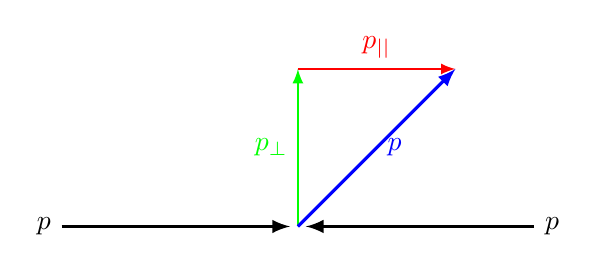
\begin{tikzpicture}
    \draw[->, black, very thick] (-3,0) node[black,left] {$p$}-- (-0.1,0){};
    \draw[->, black, very thick] (3,0) node[black,right] {$p$} -- (0.1,0){};
    \draw[->, green, thick] (0,0)-- (0,2) node[midway,left] {$\Vec{p_{\perp}}$};
    \draw[->, red, thick] (0,2)-- (2,2) node[midway,above]  {$\Vec{p_{||}}$};
    \draw[->, blue,very thick] (0,0)-- (2,2) node[midway,right]  {$\Vec{p}$};

  
\end{tikzpicture}
   % \includegraphics[width=7cm]{Figures Lecture on Datanalysis/transverse_momentum.png}
\end{center}
\end{frame}
%%%%%%%%%%%%%%%%%%%%%%%%%%%%%%%%%%%%%%%%%%%%%%%%%%%%%%%%%%%%%%%%%%%%%%%%%%%%%%%%%%%%%%%%%%%%%%
\begin{frame}{Search for $\Omega_c^0$}

  \begin{center} \vspace{-1cm}
 \Large    \[\mathbf{\Omega_c^0 \rightarrow \Xi_c^+ \, K^-}\]
 \end{center}
   \begin{spacing}{1.5}
       
  
    \begin{itemize}    \item[\ding{202}]Search for the decay products in the LHCb data 
    \item[\ding{203}]Combine the decay products and look at the mass spectrum   
        \item[\ding{204}] \textcolor{black}{We filter data}
    \item[\ding{205}] \textcolor{back}{\textbf{If we find a peak, we have discovered a new particle! }}
    \begin{itemize} %\pause
        \item [\ding{43}] \textcolor{red }{You are the scientists!}
    \end{itemize}
\end{itemize}
 \end{spacing}

\end{frame}
\begin{frame}{Summary}
We are looking for:
\begin{spacing}{1.5}
\begin{itemize}
    \item 3 tracks, identified as $p, K^-, \pi^+$
    \item These tracks originate from a secondary vertex, as the $\Xi_c^+$ flies a short distance in the detector
    \item The $\Omega_c^0$ we are looking for still decays in the $pp$ collision point (smaller IP)
    \item The desired $\Omega_c^0$ has a high transverse momentum
\end{itemize}
\end{spacing}
\end{frame}
%%%%%%%%%%%%%%%%%%%%%%%%%%%%%%%%%%%%%%%%%%%%%%%%%%%%%%%%%%%%%%%%%%%%%%%%%%%%%%%%%%%%%%%%%%%%%%
\begin{frame}{References} \footnotesize

    \begin{itemize}
\item[-] The LHCb Collaboration. Measurement of the properties of the $\Xi_b^0$ baryon. 	JHEP 1605 (2016) 161.
\item[-] The LHCb Collaboration. The LHCb Detector at the LHC.  JINST 3 (2008) S08005.
\item[-] Airbus. \url{aircraft.airbus.com/en/aircraft/a320/a321xlr#images}
\end{itemize}


    % \bibliographystyle{plain}
    % \bibliography{Z_References}
\end{frame}
%%%%%%%%%%%%%%%%%%%%%%%%%%%%%%%%%%%%%%%%%%%%%%%%%%%%%%%%%%%%%%%%%%%%%%%%%%%%%%%%%%%%%%%%%%%%%%
\end{document}

